\documentclass[11pt,a4paper]{article}

\usepackage{gastex}
\usepackage{etoolbox}
\newcommand{\showLoesung}{2} %<---als Schalter
%\newcommand{\showInhalt}{1} %<---als Schalter

\usepackage{alltt,moreverb,amsmath,enumerate}
\usepackage[normalem]{ulem}
\usepackage[T1]{fontenc}
\usepackage{ae,aecompl} %helvet,mathptm
%\usepackage[left=15mm,right=15mm,top=20mm,bottom=20mm]{geometry}
\usepackage[margin=.5in]{geometry}
%\usepackage[latin1]{inputenc} % f�r Linux
\usepackage[utf8]{inputenc} % Umlaute etc. direkt schreiben (unter Windows)
\usepackage[german]{babel}
\usepackage[url]{oth-logoPNG}
%\usepackage{i2sym,i2ams}

\usepackage{tikz}
\usetikzlibrary{arrows,shapes,trees,positioning,automata,decorations.pathreplacing,decorations.pathmorphing}
\usepackage{tkz-graph}
\usepackage{color}

\usepackage{longtable}
\usepackage{tabularx}

%\usepackage{epic}
%\usepackage{eepic}
\usepackage{comment,ifthen}
\usepackage{../include/todo}

\usepackage[T1]{fontenc}
\usepackage{textcomp}

\usepackage{listings}                   % Listings in Core-Erlang und Maude
\usepackage{lstmisc}

\usepackage{epic}                       % Bildbefehle (picture)
%\usepackage{eepic}                      % erweiterte Bildbefehle

\usepackage{bbm}                        % Mengensymbole (N,C,R,B)
\usepackage{latexsym}                   % zusaetzliche Mathesymbole
\usepackage{amsmath}                    % Mathepaket von der AMS
\usepackage{amstext}
\usepackage{amsfonts}
\usepackage{stmaryrd}                   % zusaetzliche Mathesymbole
\usepackage{mathtools}
\usepackage{amsthm}
\usepackage{cancel}

\usepackage{hyperref}
\usepackage{url}                        % Zum Setzen von URLs in typewriter-face

\pagestyle{empty}

\let\epsilon=\varepsilon
\let\phi=\varphi

\frenchspacing

\setlength{\parindent}{0pt}
\setlength{\textwidth}{18.6cm}
\setlength{\textheight}{26.5cm}
\setlength{\hfuzz}{1mm}

%%% Read dates of assignments from file
\usepackage{xparse}
\ExplSyntaxOn
\ior_new:N \g_hringriin_file_stream

\NewDocumentCommand{\ReadFile}{mm}
 {
  \hringriin_read_file:nn { #1 } { #2 }
  \cs_new:Npn #1 ##1
   {
    \str_if_eq:nnTF { ##1 } { * }
      { \seq_count:c { g_hringriin_file_ \cs_to_str:N #1 _seq } }
      { \seq_item:cn { g_hringriin_file_ \cs_to_str:N #1 _seq } { ##1 } }
   }
 }

\cs_new_protected:Nn \hringriin_read_file:nn
 {
  \ior_open:Nn \g_hringriin_file_stream { #2 }
  \seq_gclear_new:c { g_hringriin_file_ \cs_to_str:N #1 _seq }
  \ior_map_inline:Nn \g_hringriin_file_stream
   {
    \seq_gput_right:cx 
     { g_hringriin_file_ \cs_to_str:N #1 _seq }
     { \tl_trim_spaces:n { ##1 } }
   }
  \ior_close:N \g_hringriin_file_stream
 }

\ExplSyntaxOff

\ReadFile{\uebungsabgabe}{../skel/UEBUNGSABGABE.def}

%%% Read subject info from file
\newcommand{\dozent}[1]{\def\DOZENT{#1}}
\newcommand{\tutoren}[1]{\def\TUTOREN{#1}}
\newcommand{\vorlesung}[1]{\def\VORLESUNG{#1}}
\newcommand{\semester}[1]{\def\SEMESTER{#1}}

\InputIfFileExists{../skel/VORLESUNG.def}{\providecommand{\TUTOREN}{}}%
{\typeout{***********}
 \typeout{Warnung: Kein File vorhanden, das die Vorlesung spezifiziert!}
 \typeout{Spezifikation muss daher im Text des Blattes oder ueber die
          Tastatur erfolgen.}
 \typeout{***********}}

\def\Uebung#1#2#3{
  \othLehrstuhlLogo[\DOZENT]
  \begin{center}
	{~\\[-2em]\Large\bf \VORLESUNG}\\[0.5em]
    \LARGE --~Tutorium #1 (Übung #2)~--\\[4mm]
  \
  \normalsize
  \textbf{#3}
    \rule{\textwidth}{0.1pt}\\[1cm]
  \end{center}
}

\def\Hinweis#1{
	{~\\[-3em]\bf Hinweis: }
	\begin{minipage}[t]{16.5cm}
	#1
	\end{minipage}\\[1em]
    \rule{\textwidth}{0.1pt}
}

\def\Tipps#1{
	{~\\[-3em]\bf Tipps: }
	\begin{minipage}[t]{16.5cm}
	#1
	\end{minipage}\\[1em]
    \rule{\textwidth}{0.1pt}
}
  
\def\MyHeader{
  \othLehrstuhlLogo[Prof.~Dr.~rer.~nat.~Carsten~Kern]%[Carsten~Kern,~Stefan~Rieger]
}

\newcommand{\sem}[1]{[\![#1\,]\!]}

\def\aufgabe#1#2{\subsection*{Aufgabe #1 (#2)}\par}
\def\endaufgabe{}

\newenvironment{loesung}{\subsection*{L\"osungsvorschlag:}}{}
\newenvironment{hinweis}{}{}
\ifthenelse{\isundefined{\showLoesung}}{\excludecomment{loesung}}{\pagestyle{plain}\excludecomment{hinweis}}

\newenvironment{tipps}{}{}
\ifthenelse{\isundefined{\showTipps}}{\excludecomment{tipps}}{\excludecomment{hinweis}}

\newenvironment{inhalt}{\subsection*{Kommentar:}}{}
\ifthenelse{\isundefined{\showInhalt}}{\excludecomment{inhalt}}{}

\long\def\Exercise#1#2{\begin{exercise}{#1}#2\end{exercise}}

\def\underbar#1{%
  \setbox0=\hbox{#1}%
  \dimen0=\dp0\relax%
  \dp0=0pt%
  \setbox0=\hbox{\underline{\box0}}%
  \dp0=\dimen0\relax%
  \box0%
  }

\makeatletter
\def\@makeunderbar[#1]#2{\expandafter\def\csname#1\endcsname{\underbar{#2}}}
\def\makeunderbar{\@ifnextchar[{\@makeunderbar}{\@makeunderbar[]}}
\makeatother

\def\T{\mathrm{T}}
\def\P{\mathrm{P}}
\def\CT{\mathrm{CT}}
\def\COp{\mathrm{COp}}

\makeunderbar{Comp}
\makeunderbar{Ops}
\makeunderbar{trans}
\makeunderbar[strans]{s-trans}
\makeunderbar[ntrans]{n-trans}
\makeunderbar{fix}

\def\labelenumi{\alph{enumi})}
\let\<=\langle
\let\>=\rangle

\parindent=0pt
\parskip=1ex

\definecolor{javared}{rgb}{0.6,0,0} % for strings
\definecolor{javagreen}{rgb}{0.25,0.5,0.35} % comments
\definecolor{javapurple}{rgb}{0.5,0,0.35} % keywords
\definecolor{javadocblue}{rgb}{0.25,0.35,0.75} % javadoc
 
\lstset{language=C++,
basicstyle=\ttfamily\footnotesize,
keywordstyle=\color{javapurple}\bf,
stringstyle=\color{javared},
commentstyle=\color{javagreen}\it\bf,
morecomment=[s][\color{javadocblue}]{/**}{*/},
numbers=left,
numberstyle=\tiny\color{gray},
stepnumber=1,
numbersep=10pt,
tabsize=3,
showspaces=false,
showstringspaces=false}

\usepackage{enumitem}
\usepackage{algpseudocode}
\usepackage{caption}
\usepackage{subcaption}
\usepackage{placeins}
\usepackage{multicol}

\begin{document}
\thispagestyle{empty}

\Uebung{6}{7}{Simon Thelen}{18. November 2021}  % FIXME: Blattnummer, Datum, Zeit

%%%%%%%%%%%%%%%%%%%%%%%%%%%%%%%%%%%%%%%%%%%%%%%%%%%%%%%%%%%%%%%%%%%%%%

\ifcsdef{showLoesung}{
\textbf{Bitte beachten Sie:} Die Lösungen können trotz sorgfältiger Prüfung Fehler enthalten.
Bei Fragen oder Unklarheiten kontaktieren Sie bitte den Tutor oder Dozenten in Tutorien, Übungen oder nach Vorlesungen.
}{}


\begin{aufgabe}{1}{Binäre, verkettete Bäume}
    \begin{enumerate}
        \item Gegeben sei ein binärer, verketteter Baum mit Preorder-Darstellung (a, b, c, d, e, f, g, h, i) und Inorder-Darstellung (c, d, b, e, a, h, g, i, f).
        Wie sieht der Baum aus?
        \item Angenommen Sie haben die Preorder- und die Postorder-Darstellung eines binären Baumes gegeben.
        Können Sie (wie bei der vorherigen Teilaufgabe) den Baum eindeutig rekonstruieren?
        Falls ja, begründen Sie dies.
        Falls nein, geben Sie ein Gegenbeispiel an.
        \item Betrachten Sie folgende Implementierung eines Inorder-Durchlaufs über einen binären, verketteten Baum:
        \begin{lstlisting}[language=c++]
void inorder(Node *node) {
    if (node->left != NULL) inorder(node->left);
    cout << node->value << " ";
    if (node->right != NULL) inorder(node->right);
}
        \end{lstlisting}
        Begründen Sie, dass die Laufzeit dieser Funktion für einen Baum mit $n$ Elementen $O(n)$ beträgt, indem Sie einen Zusammenhang zwischen Kanten des Baumes und den rekursiven Aufrufen des Algorithmus herstellen.   
        % \item
        % Implementieren Sie einen Preorder-Durchlauf über einen binären, verketten Baum (in Pseudocode oder einer Programmiersprache Ihrer Wahl), der auf Rekursion verzichtet, aber stattdessen einen Stack verwendet.
        \item 
        Geben Sie einen Algorithmus in Pseudocode oder einer Programmiersprache Ihrer Wahl an, welcher einen binären, verketteten Baum schichtweise ausgibt.
        Also zunächst den Wurzelknoten, dann die Kindknoten der Wurzel von links nach rechts, dann alle Enkelknoten der Wurzel von links nach rechts und so weiter.
        \begin{description}
            \item[Tipp:] Verwenden Sie eine Queue.
        \end{description}
        \item
        Der Abstand von zwei Knoten in einem Baum ist die Anzahl an Kanten, die mindestens traversiert werden müssen, um von einem Knoten zum anderen zu gelangen.
        \emph{Beispiel:} Die Knoten 3 und 13 im Baum aus Aufgabe 2\ref*{insert_delete} haben Abstand 6.

        Geben Sie einen Algorithmus in Pseudocode oder einer Programmiersprache Ihrer Wahl an, welcher einen binären, verketteten Baum als Eingabe erhält und den größten Abstand von zwei Knoten im Baum liefert.
        Eine einfache Lösung hat Laufzeit $O(n^2)$.
        Schaffen Sie es sogar in $O(n)$?
    \end{enumerate}
\end{aufgabe}
\begin{loesung}
    \begin{enumerate}
        \item \ \\
        \begin{figure}[h!]
            \centering
            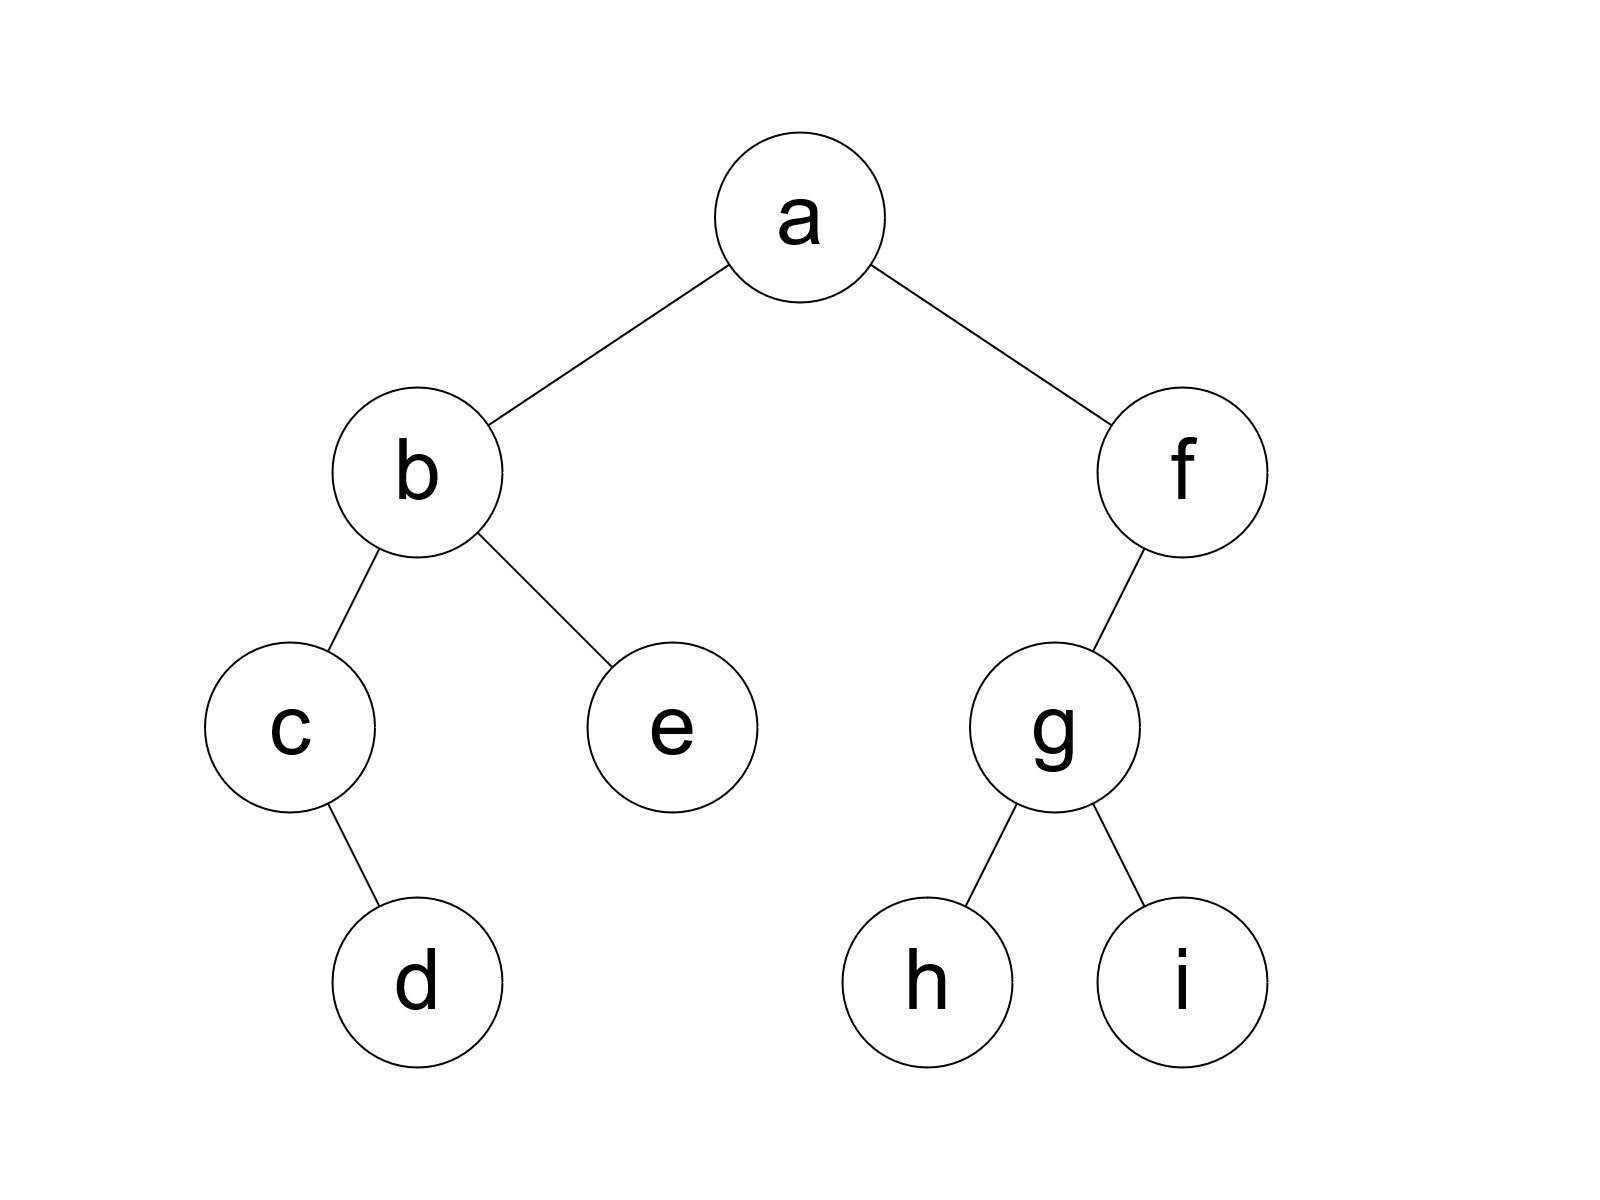
\includegraphics[width=0.3\textwidth]{img/1a}
        \end{figure}
        \FloatBarrier
        \item Eine eindeutige Rekonstruktion ist allein bei gegebener Preorder- und Postorder-Darstellung im Allgemeinen nicht möglich.
        Das kleinste Gegenbeispiel sind die folgenden, beiden Bäume:
        \begin{figure}[h!]
            \centering
            \begin{subfigure}[b]{0.23\textwidth}
                \centering
                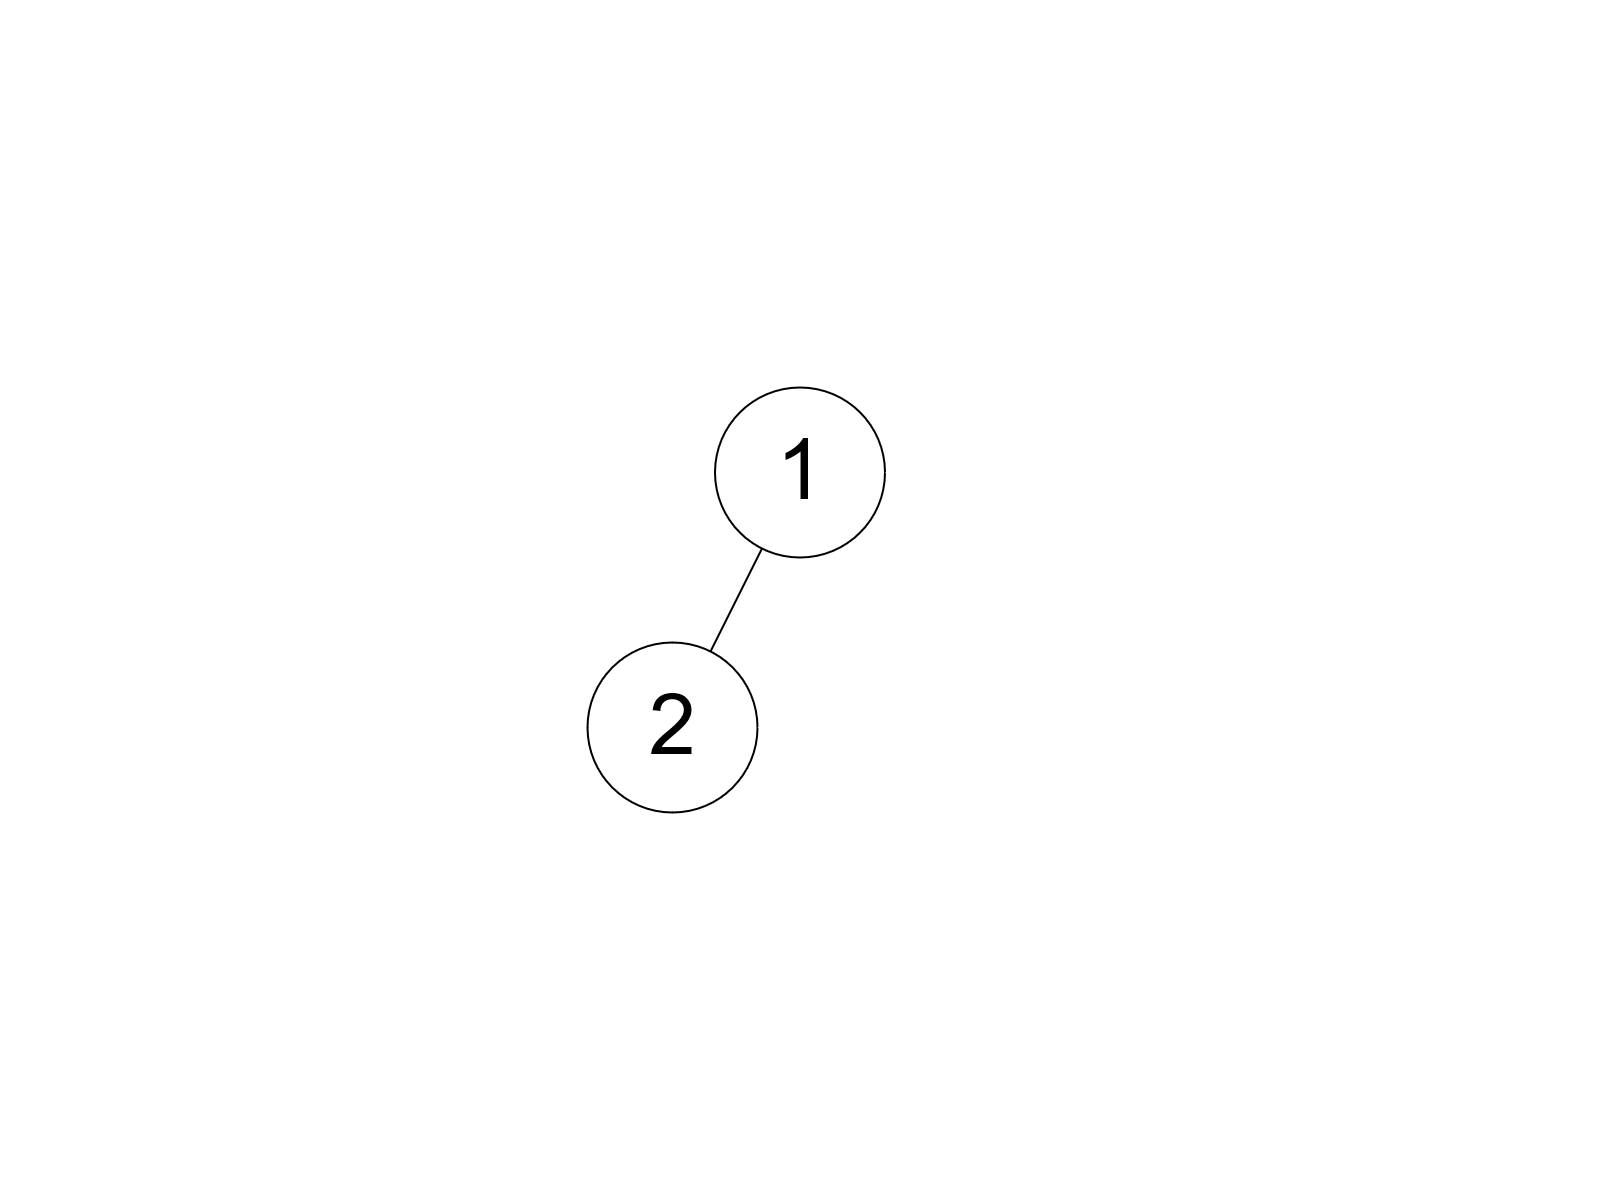
\includegraphics[width=\textwidth]{img/1b_1}
            \end{subfigure}
            \begin{subfigure}[b]{0.23\textwidth}
                \centering
                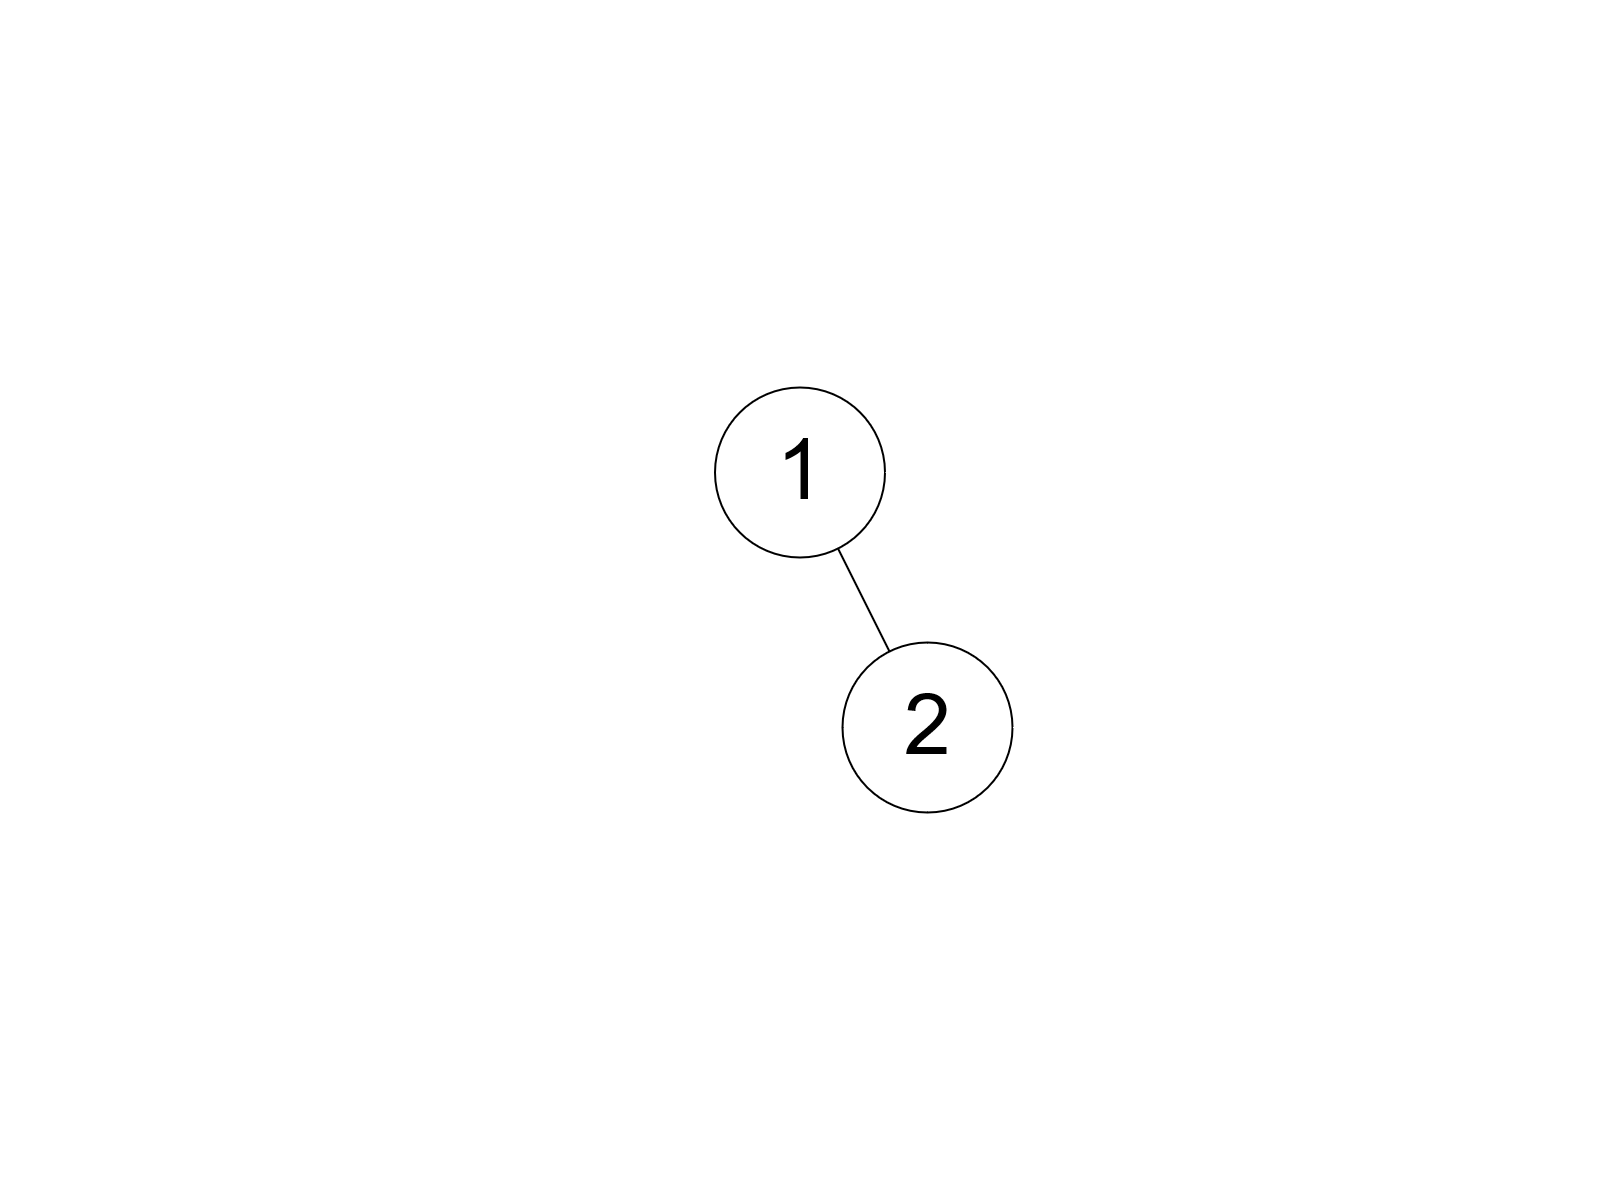
\includegraphics[width=\textwidth]{img/1b_2}
            \end{subfigure}
        \end{figure}
        \FloatBarrier
        Beide haben Preorder-Darstellung (1, 2) und Postorder-Darstellung (2, 1).

        Das gleiche gilt für andere entartete Bäume (Bäume, bei denen jeder Knoten maximal einen Nachfolger hat).
        Nummeriert man die Knoten eines entarteten Baumes mit $n$ Knoten von Wurzel zum Blatt durch, hat der Baum die Preorder-Darstellung (1, 2, $\ldots$, $n - 1$, $n$) und Postorder-Darstellung ($n$, $n - 1$, $\ldots$, 2, 1).
        Das gilt für alle entarteten Bäume mit gleich vielen Knoten, obwohl es insgesamt $2^n$ solcher Bäume gibt.

        \item
        Jeder Binärbaum ist zusammenhängend.
        Das heißt, alle Knoten des Baumes werden erreicht.
        Jeder Binärbaum ist außerdem zyklenfrei.
        Das bedeutet, dass kein Knoten doppelt untersucht wird (es gibt keine Kante, die nach oben im Baum führt).
        Daraus folgt, dass für jede der $n - 1$ Kanten des Baumes genau ein rekursiver Aufruf von \texttt{inorder} durchgeführt wird.
        Dazu kommt noch der initiale Aufruf auf die Wurzel des Baumes.
        Macht insgesamt $n$ Aufrufe.
        Jeder Aufruf benötigt offensichtlich nur konstante Laufzeit.
        Die Laufzeit eines Inorder-Durchlaufs beträgt daher $O(n)$.

%         Angenommen, die Implementierung sähe aus:
%         \begin{lstlisting}[language=c++]
% void inorder(Node *node) {
%     if (node == NULL) return;
%     inorder(node->left);
%     cout << node->value << " ";
%     inorder(node->right);
% }
%         \end{lstlisting}
%         Hier werden die Prüfungen auf \texttt{NULL} sozusagen auf die nächsttiefere Rekursionsebene verschoben.
%         Die Laufzeit ist augenscheinlich größer, da mehr rekursive Aufrufe nötig sind.
%         Andererseits ist leicht zu sehen, dass der Algorithmus praktisch identisch zur ursprünglichen Variante ist.
        \item Die Idee ist, zunächst nur den Wurzelknoten in dei Queue einzufügen und anschließend über alle Knoten in der Queue zu iterieren.
        Jedes Knoten, der untersucht wird, wird aus der Queue entfernt und ausgeben.
        Anschließend werden alle Nachfolger des Knotens (von links nach rechts) in die Queue eingefügt.
        \begin{lstlisting}[language=c++]
void layerTraversal(Tree *tree) {
    queue q(tree->n);
    if (tree->root != NULL) q.enqueue(tree->root);
    while (!q.isEmpty()) {
        Node *node = q.dequeue();
        cout << node->value << " ";
        if (node->left != NULL) q.enqueue(node->left);
        if (node->right != NULL) q.enqueue(node->right);
    }
}            
        \end{lstlisting}
        Man kann sich überlegen, dass in dem Moment, wenn alle Knoten aus Schicht $k$ abgearbeitet wurden, die Queue genau die Knoten aus Schicht $k + 1$ enthält und zwar von links nach rechts.
        \begin{proof}
            Beweis durch vollständig Induktion über die Anzahl der Schichten
            \begin{description}
                \item[IA] Zu Beginn ist nur der Wurzelknoten in der Queue.
                Im ersten Schleifendurchlauf wird dieser aus der Queue entfernt und seine Nachfolger von links nach rechts eingefügt.
                Die Aussage ist also für Schicht 1 korrekt. 
                \item[IV] Sei die Aussage wahr für $k - 1$.
                \item[IS]
                Dann werden durch das FIFO-Prinzip der Queue alle Knoten aus Schicht $k$ von links nach rechts abgearbeitet, bevor Knoten aus tieferen Schichten untersucht werden.
                Da außerdem für jeden Knoten seine Nachfolger von links nach rechts in die Queue eingefügt werden, liegen, nachdem alle Knoten aus Schicht $k$ untersucht wurden, alle Knoten aus Schicht $k + 1$ von links nach rechts in der Queue.
                Da zu untersuchende Knoten aus der Queue entfernt werden und aufgrund der Induktionsvoraussetzung keine anderen Knoten in der Queue liegen können, liegen, nachdem die Knoten aus Schicht $k$ untersucht wurden, genau die Knoten aus Schicht $k + 1$ in der Queue und zwar von links nach rechts.
            \end{description}
            Nach dem Prinzip der vollständigen Induktion gilt obige Aussage für alle $k$.
        \end{proof}
        Aus der gerade bewiesen Aussage folgt, dass alle Knoten des Baumes schichtweise durchlaufen und somit ausgegeben werden.

        Da jeder Knoten genau einmal in die Queue eingefügt wird und pro Knoten in der Queue konstanter Zeitaufwand besteht, ist die Laufzeit des obigen Algorithmus $O(n)$.

        Der beschriebene Algorithmus entspricht einer Breitensuche (Breadth First Search).
        Diese wird später in der Vorlesung näher behandelt.

        \item
        Der größte Abstand zweier Knoten entspricht dem längsten (einfachen, also zyklenfreien) Pfad zwischen zwei Knoten im Baum.
        Es soll über alle Knoten iteriert werden und für jeden Knoten die Länge des längsten Pfades im Teilbaum unter diesem gefunden werden.
        Die Länge des längsten Pfades im Teilbaum unter dem Wurzelknoten ist die gesuchte Antwort.
        Dabei gilt für jeden Knoten, dass der längste Pfad im entsprechen Teilbaum
        \begin{enumerate}[label=\arabic*.]
            \item sich entweder im Teilbaum unter dem linken Nachfolger befindet,
            \item sich im Teilbaum unter dem rechten Nachfolger befindet
            \item oder durch den Knoten selbst läuft.
        \end{enumerate}
        Die ersten beiden Fällen können durch die Rekursion abgedeckt werden, die beim Durchlaufen des Baumes sowieso nötig ist.
        Anschließend wird der dritte Fall behandelt:
        Der längste Pfad durch den Knoten startet im linken Teilbaum und zwar so weit unten wie möglich, läuft hoch bis zum Knoten und dann in den rechten Teilbaum, wieder so tief wie möglich.
        Der Abstand vom einem Knoten zum \glqq{}tiefsten\grqq{} Kind ergibt sich die Höhe des Teilbaums:
        \begin{lstlisting}[language=c++]
int height(Node *node) {
    if (node == NULL) return -1;
    return 1 + max(height(node->left), height(node->right));
}
        \end{lstlisting}
        Es wird also die Höhe des linken und die des rechten Teilbaumes berechnet.
        Dazu kommen noch die zwei Kanten \glqq{}Wurzel linker Teilbaum zum Knoten\grqq{} und \glqq{}Knoten zur Wurzel rechter Teilbaum\grqq{}.
        Die Länge des Pfades ergibt sich also durch \texttt{2 + height(left) + height(right)}.
        \begin{lstlisting}[language=c++]
int maxDistance(Node *node) {
    if (node == NULL) return INT_MIN;
    return max(
        max(maxDistance(node->left), maxDistance(node->right)),
        2 + height(node->left) + height(node->right)
    );
}
int maxDistance(Tree *tree) {
    return maxDistance(tree->root);
}
        \end{lstlisting}
    \end{enumerate}
    Pro Knoten wird die Laufzeit von den beiden \texttt{height}-Aufrufen dominiert.
    Die Wurzel benötigt den größten zeitlichen Aufwand, da die beiden \texttt{height}-Aufrufe zusammen den gesamten restlichen Baum durchlaufen, was Zeitaufwand $\Theta(n)$ allein für die Wurzel bedeutet.
    Da es insgesamt $n$ Knoten gibt, beträgt der Gesamtaufwand für den Algorithmus $O(n^2)$.
    Dieser wird in der Praxis auch tatsächlich erreicht (Es ist leicht zu sehen, dass die Laufzeit bei einem entarteten Baum durch die Gauß-Summe gegeben ist).

    Die wesentliche Überlegung, um Gesamtlaufzeit $O(n)$ zu erreichen, ist, dass Höhe und maximale Distanz der Teilbäume parallel berechnet und anschließend zwischengespeichert werden kann, um sich unnötige, doppelte Berechnungen zu sparen.
    \begin{lstlisting}[language=c++]
int maxDistanceLinear(Node *node, int &height) {
    if (node == NULL) {
        height = -1;
        return INT_MIN;
    }
    int leftHeight, rightHeight;
    int result = std::max(
        maxDistanceLinear(node->left, leftHeight),
        maxDistanceLinear(node->right, rightHeight)
    );
    height = 1 + std::max(leftHeight, rightHeight);
    return std::max(result, 2 + leftHeight + rightHeight);
}
int maxDistanceLinear(Tree *tree) {
    int height;
    maxDistanceLinear(tree->root, height);
}
    \end{lstlisting}
    In dieser Lösung wird die maximale Distanz per \texttt{return} zurückgegeben und die Höhe mittels Referenz-Parameter \texttt{height}.
    Pro Knoten ist abgesehen von den rekursiven Aufrufen nur noch konstante Laufzeit nötig.
    Heißt, die Gesamtlaufzeit beträgt nun $O(n)$.
\end{loesung}

\begin{aufgabe}{2}{Binäre, verkettete Suchbäume}
    \begin{enumerate}[label=\alph*)]
        \item Gegeben sei ein binärer, verketteter Suchbaum mit Postorder-Darstellung (15, 28, 12, 33, 41, 37, 30, 50, 42).
        Wie sieht der Baum aus?
        % Quelle: Cormen 12.2-1
        \item Angenommen, Sie suchen den Wert 75 in einem binären, verketteten Suchbaum.
        Welche der folgenden Pfade von der Wurzel bis zum gesuchten Knoten ist nicht möglich: (51, 52, 97, 80, 72, 76, 75) oder (89, 80, 24, 63, 81, 69, 75)?
        Begründen Sie Ihre Entscheidung.
        \item Gegeben seien die Werte (29, 33, 45, 50, 77, 86, 96).
        Geben Sie binäre, verkette Suchbäume mit Höhe 2, 3, 4, 5 und 6 an, die jeweils genau diese Elemente enthalten.
        \item\label{insert_delete} Gegeben sei folgender binärer, verketteter Suchbaum:
        \begin{figure}[h!]
            \centering
            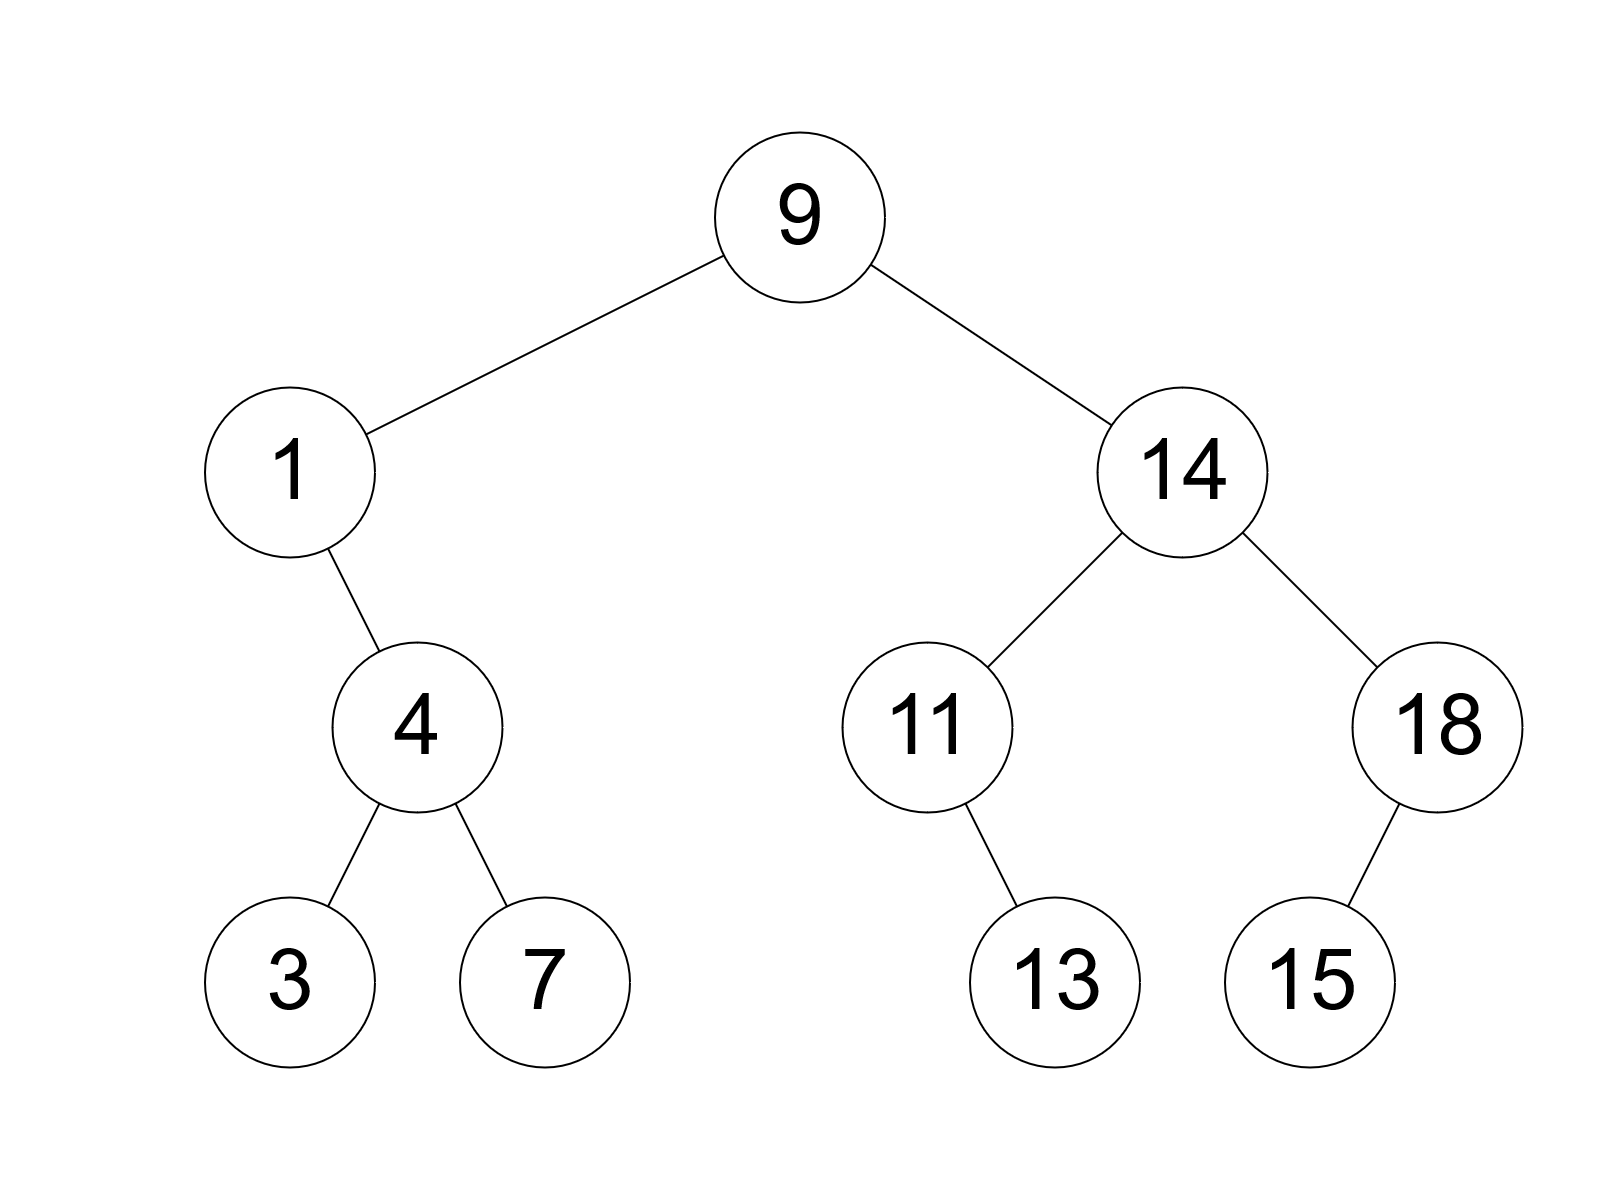
\includegraphics[width=0.3\textwidth]{img/2d}
        \end{figure}
        \FloatBarrier
        \ \\
        Führen Sie nacheinander folgende Operationen durch: \textsc{Delete(15), Delete(1), Delete(9), Insert(1), Insert(12)}.
        Geben Sie alle Zwischenschritte an.
        \item 
        Geben Sie einen Algorithmus in Pseudocode oder einer Programmiersprache Ihrer Wahl an, der einen binären, verketteten Suchbaum sowie zwei Werte $l$ und $h$ als Eingabe erhält und anschließend alle Werte $x$ des Baumes ausgibt, für die $l \leq x \leq h$ gilt.
        Versuchen Sie so gut wie möglich, nur selektiert über den Teil des Baumes zu iterieren, der für die Ausgabe relevant ist.
    \end{enumerate}
\end{aufgabe}

\begin{aufgabe}{3}{AVL-Bäume}
    \begin{enumerate}
        \item Gegeben sei folgender AVL-Baum:
        \begin{figure}[h!]
            \centering
            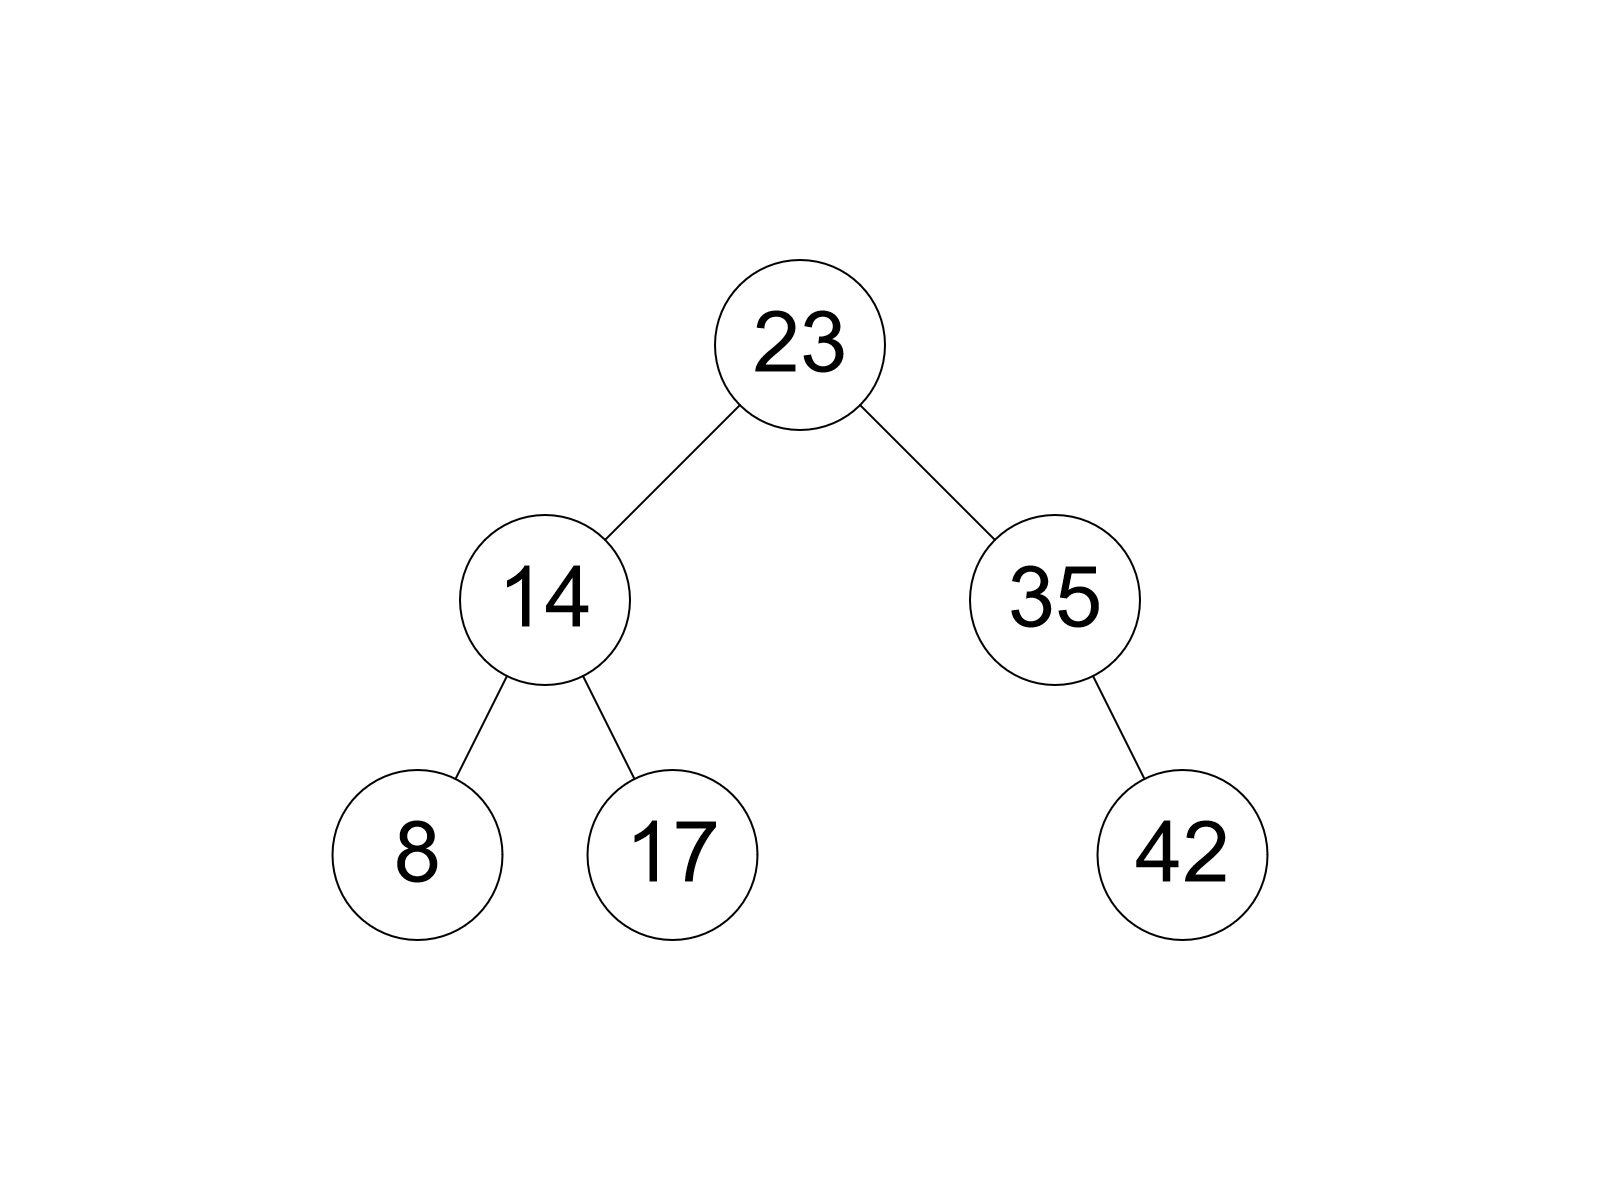
\includegraphics[width=0.3\textwidth]{img/3a}
        \end{figure}
        \FloatBarrier
        \ \\
        Führen Sie nacheinander folgende Operationen durch: \textsc{Insert(5), Insert(3), Insert(38), Insert(2), Delete(3), Delete(38), Delete(42)}.
        Geben Sie alle Zwischenschritte und Rotationen an.
        % Quelle: Cormen Aufgabe 12.1-1
        \item Begründen Sie oder widerlegen Sie die folgende Aussage:
        \begin{center}
            \emph{Bei jedem }\textsc{Insert}\emph{-Aufruf ist maximal eine (Doppel-)Rotation notwendig}
        \end{center}
        \item Geben Sie ein Beispiel für das Löschen eines Knotens an, bei dem mehr als eine (Doppel-)Rotation benötigt wird.
        \begin{description}
            \item[Tipp:] Sie können zum Beispiel den minimalen AVL-Baum der Höhe 4 verwenden.
        \end{description}
        \item Implementieren Sie die folgenden Operationen, die Sie im Rahmen der Heap-Datenstruktur kennen gelernt haben, mithilfe eines AVL-Baumes (in Pseudocode oder einer Programmiersprache Ihrer Wahl).
        Geben Sie außerdem an, wie Sie die AVL-Datenstruktur aus der Vorlesung erweitern müssen, um die angegebenen Laufzeiten zu erreichen.
        \begin{table}[h!]
            \centering
            \begin{tabular}{|l|l|l|}
            \hline
            \multicolumn{1}{|c|}{\textbf{Operation}}  & \multicolumn{1}{c|}{\textbf{Laufzeit}} & \multicolumn{1}{c|}{\textbf{Beschreibung}}\\ \hline
            \textsc{GetMaximum} & $O(1)$      & Gibt den größten Wert im Baum zurück.\\ \hline
            \textsc{ExtractMax} & $O(\log n)$ & Entfernt den größten Wert aus dem Baum. \\ \hline
            \textsc{Insert}     & $O(\log n)$ & Fügt einen neuen Wert in den Baum ein. \\ \hline
            \end{tabular}
        \end{table}
    \end{enumerate}
\end{aufgabe}

\begin{loesung}
    \begin{enumerate}
        \item \ \\
        \begin{figure}[h!]
            \centering
            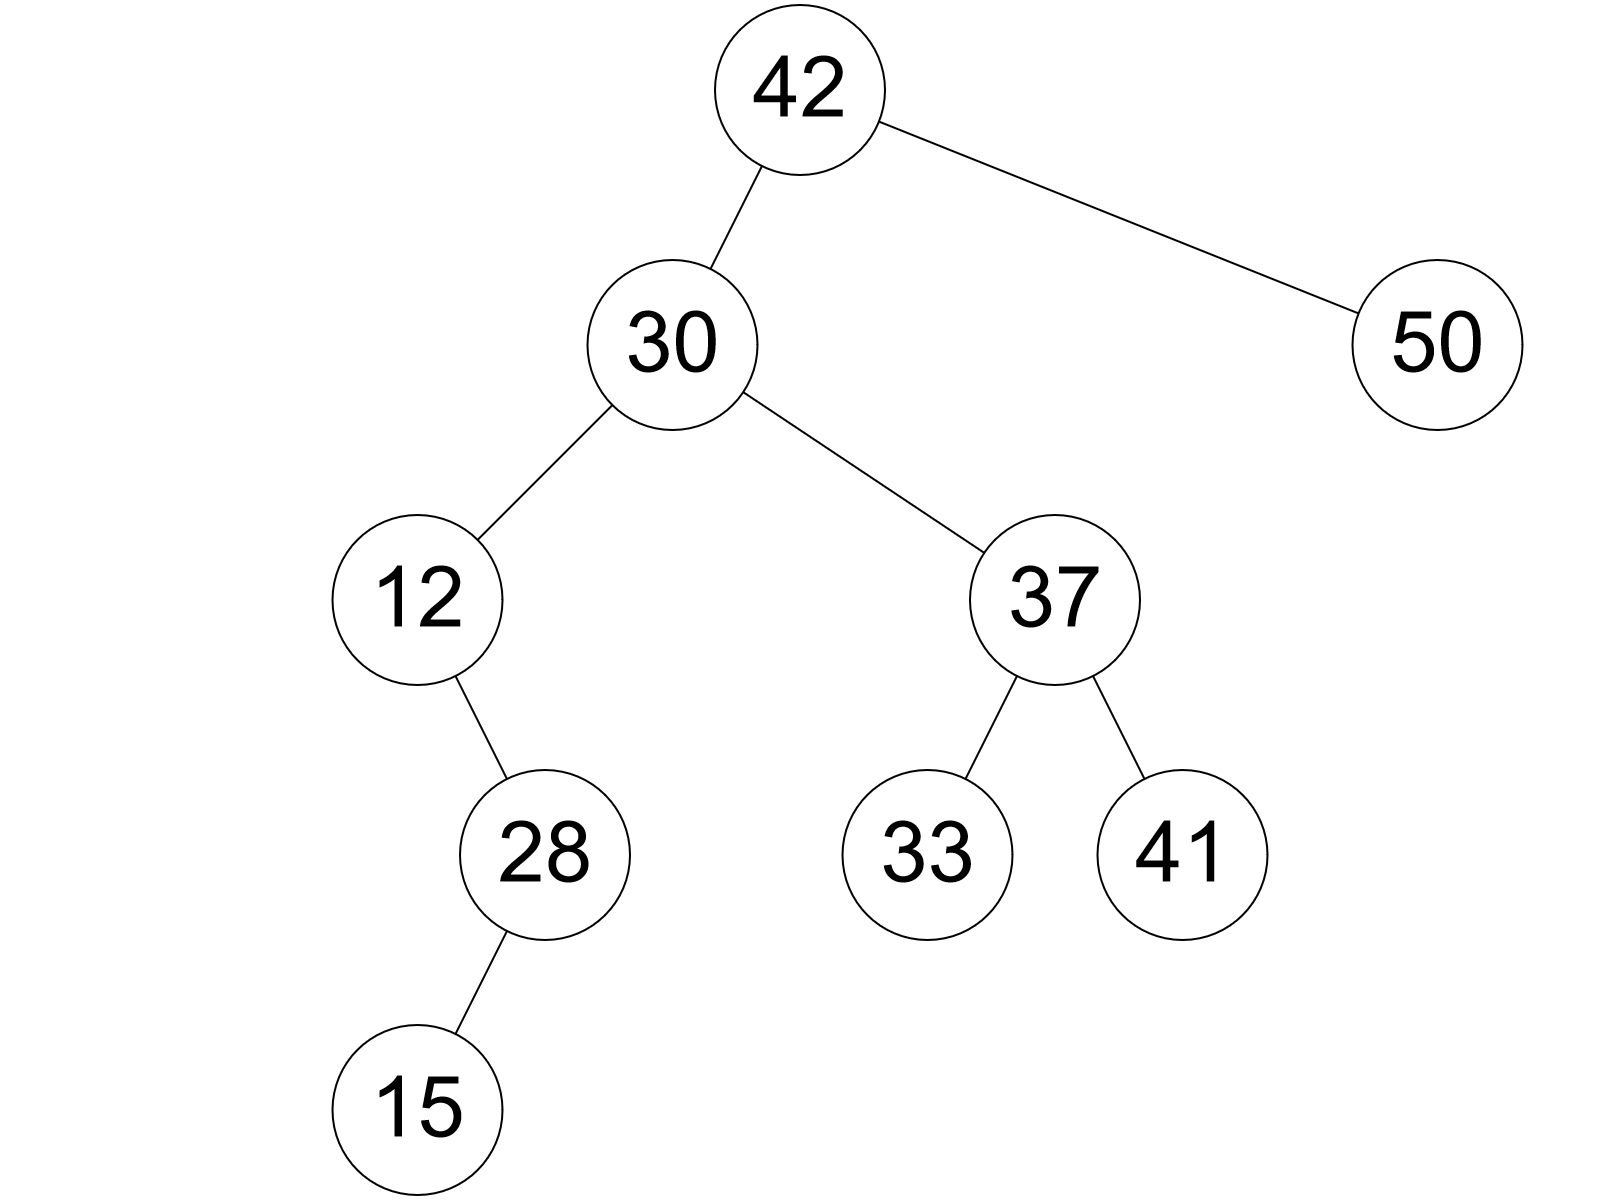
\includegraphics[width=0.3\textwidth]{img/2a}
        \end{figure}
        \FloatBarrier
    \end{enumerate}
\end{loesung}


\end{document}